\chapter{Experimental Design}

To test the effect of a barrier's height on the probability of tunneling, I used a combination of procedures and conventions from the experiments of John Bush, Yves Couder, and specifically, Eddi 2009 (CITE!). These elements were then slightly modified to fit some of the unique features of my experiment. In particular, I aim to give some of the reasoning behind the tray design and data collection techniques, both of which are not well described in the literature.

\section{Materials}
The key materials of this experiment are the shaker, the oil, and the tray. In this section I'll describe the specifics of the big three, as well as some of the additional components used in data collection. 

\subsection{Tray}
The tray was made of plastic parts machined by the laser cutter. They were then glued together with GLUE?. The tray's design guides the droplet and creates smooth droplet trajectories. The tray schematic is shown in \refFig{tray}. 

\begin{figure}[h!]
	\centering
	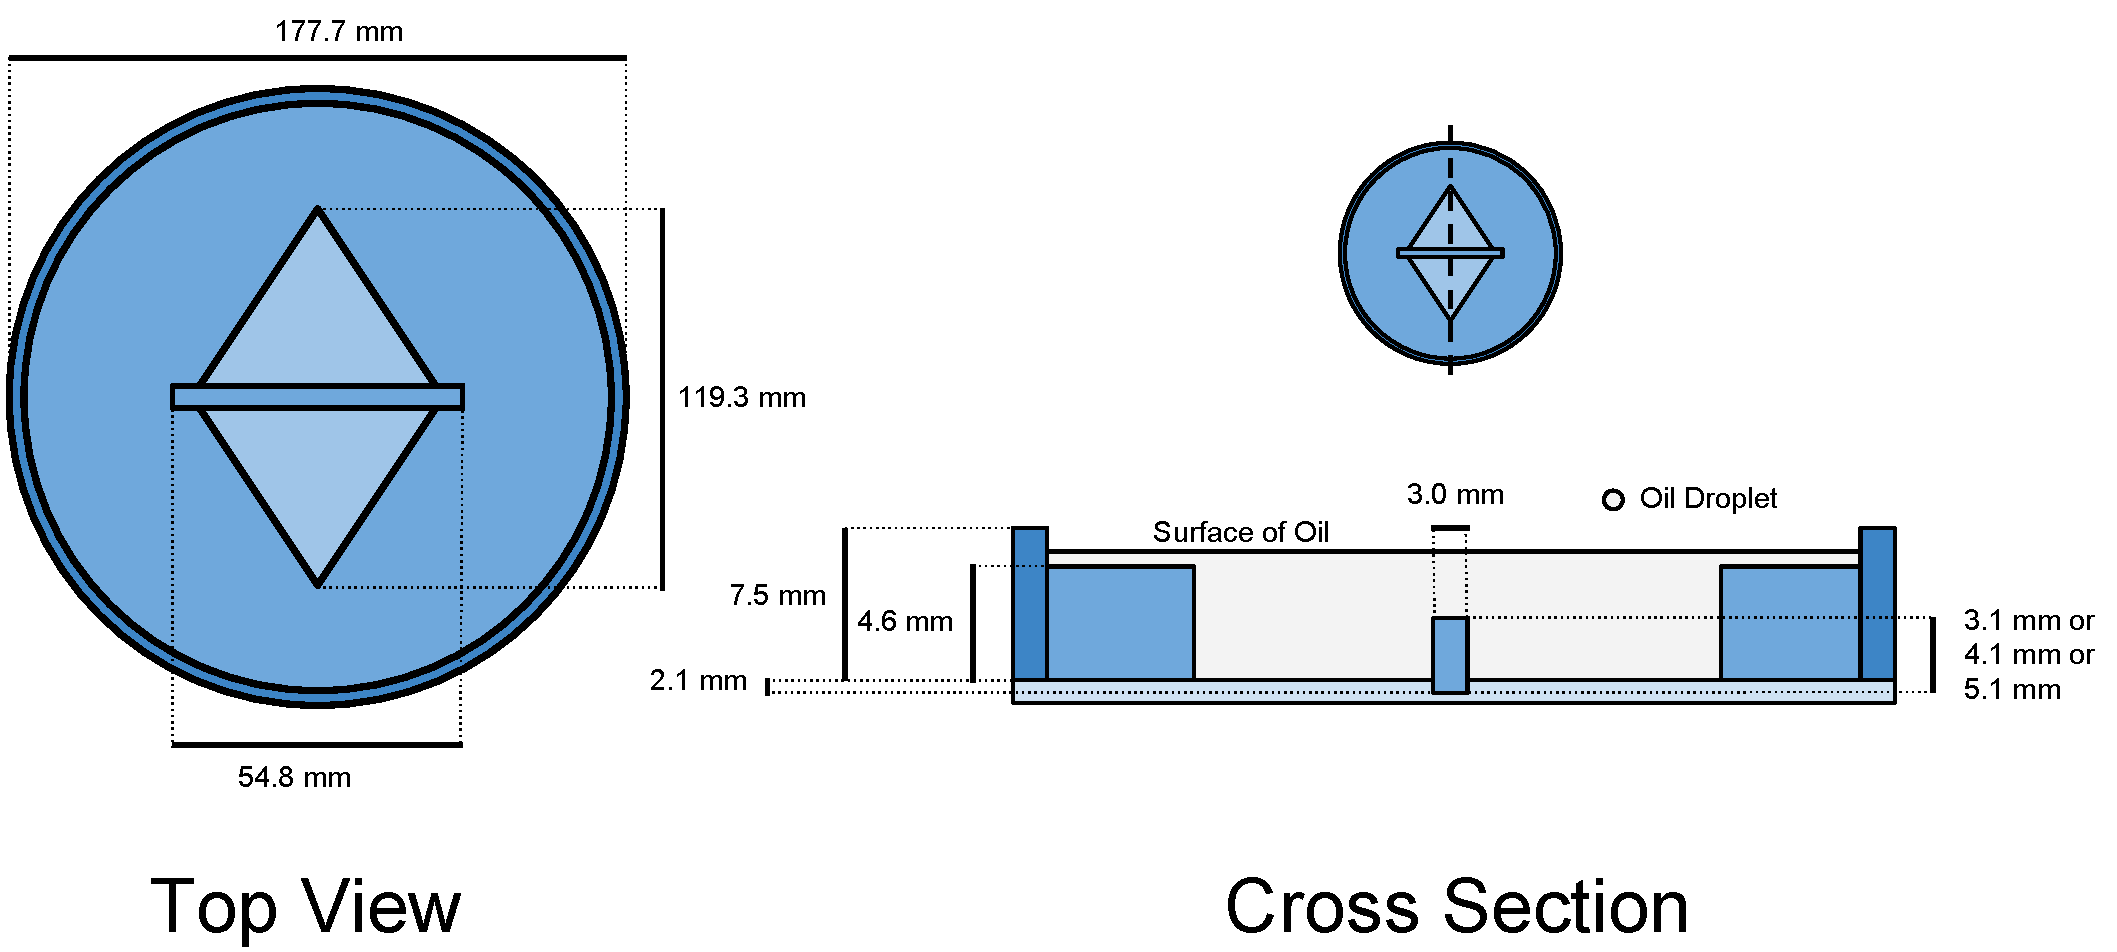
\includegraphics[scale=0.48]{Tray.pdf}
	\caption{The specifications of the tray design. The top view (left) highlights the main elements in the tray, while the cross section (rignt) illustrates the topography of the tray.}
	\label{tray}
\end{figure}

A thin layer of oil spills over the constraining rhombus shape. As long as the layer is thin enough, the droplet will remain in the rhombus container, but the waves will continue to propogate unimpeded. This gives the waves time to decay, and means that the droplets motion isn't chaotically affected by reflections of previous waves and is instead guided by the unreflected waves. 

The rhombus shape serves to steer the droplet into a perpendicular collision with the barrier. This works because the droplet will find its way into the acute corner of the rhombus, and will shoot out, pinballing off of the edges of the rhombus until settling into a straight line, directly towards the barrier.  FIGURE?

I designed my experiment to test barriers of three different heights: $1~\mathrm{mm}$, $2~\mathrm{mm}$, and $3~\mathrm{mm}$, measured from the surface of the rhombus. Due to the nature of the plastic and the laser cutter, manufacturing a barrier with a height of $1~\mathrm{mm}$ would inevitably bend. The solution to this problem was to make these barriers taller, and create an cut-out in the rhombus so they could be inserted. The cut outs were deep enough to exactly counter the added height of the barrier, so the barriers still had (when measured from the surface of the rhombus) heights of $1~\mathrm{mm}$, $2~\mathrm{mm}$, and $3~\mathrm{mm}$. This also solved the problem of fixing the barriers in place, without disturbing the floor. 


The bottom of the tray was painted black in order to provide contrast, which allows the droplet to be more easily tracked by eye and by camera.





\subsection{Silicon Oil}
    The silicone oil used in this experiment had a viscocity of 20 cSt (the thickness is a little closer to water than olive oil) obtained from Clearco Products Co., Inc. (CAS No: 63148-62-9). The 20 cSt viscocity of Bush's group was used (over the 50 cSt viscocity of Courder's) because it seems to be developing as the standard in this subfield. The tray requires about a quarter of a pint of the fluid.
    
    It is of vital importance to keep the oil as clean as possible because it keeps the droplet bouncing for longer. This means protecting both from particulate matter that is already in the tray and from the particulate matter that might float on to the surface of the oil. The first problem was tackled by thoroughly cleaning the tray immediately before use. The second problem was mitigated in two steps: first, the experiment was done as soon as possible after the oil was initially poured into the tray; and second, a shield was placed over the tray to block dust.     

\subsection{Windshield}
    A large, see-through cylinder (covered at one end) was manufactured by the laser cutter. When placed over the tray, it served the purpose of keeping the oil clean from particulate matter and preventing wind currents from influencing the motion of the walker. 

\subsection{Shaker}

\subsection{Accelerometer}  
    Knowing the tray's acceleration allows us to characterize the behaviour of our system using \refFig{regime}. To measure acceleration, we attached an ADLX 326 triple axis accerlerometer to the bottom of the tray. The method of attachement was screws, since it provided a much firmer yet more removable hold than tape or glue. The accerlerometer has a range of $\pm$16$g$, perfect for measuring the accelerations in our setup, which average about 5$g$'s. 
      
      The signal from the z-axis of the accelerometer was output directly into the oscilloscope. For the vibrating tray, the output was approximately sinusoidal (as expected). The spec sheet for the accelerometer indicates that the sensitivity can be translated to $57 \pm 6~\mathrm{mV/g}$. 

\subsection{Camera} 

\subsection{Other}
    The speaker was driving with a wave generator NAME, amplified by an amplifier, NAME.    
 
\section{Setup}
    The combined setup is shown in \refFig{setup}.
    
\begin{figure}[h!]
	\centering
	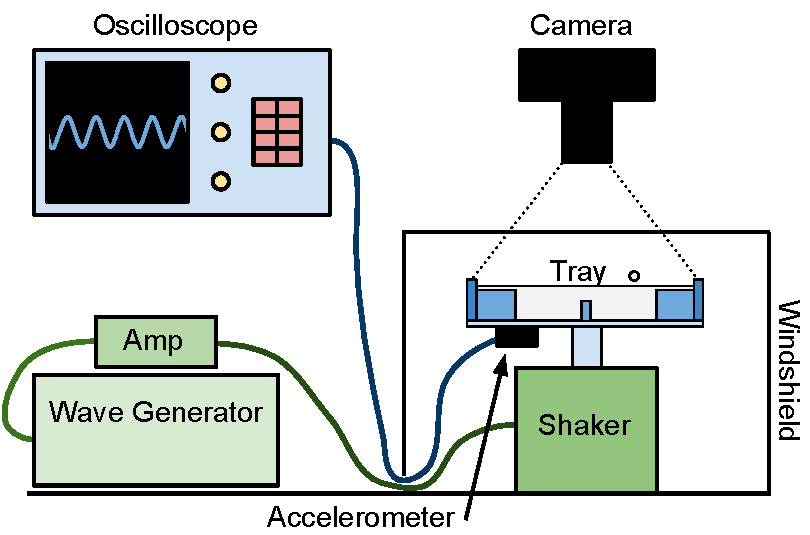
\includegraphics[scale=0.8]{Setup.pdf}
	\caption{The experimental setup. The amplified signal from the wave generator drives the shaker. The accelerometer generates a signal which is read by the oscilloscope. The windshield blocks disturbances to the experiment, while allowing the camera to document the trials.}
	\label{setup}
\end{figure}

\section{Data Collection}

